%%%%%%%%%%%%%%%%%%%%%%%%%%%%%%%%%%%%%%%%%
% Journal Article
% LaTeX Template
% Version 1.4 (15/5/16)
%
% This template has been downloaded from:
% http://www.LaTeXTemplates.com
%
% Original author:
% Frits Wenneker (http://www.howtotex.com) with extensive modifications by
% Vel (vel@LaTeXTemplates.com)
%
% License:
% CC BY-NC-SA 3.0 (http://creativecommons.org/licenses/by-nc-sa/3.0/)
%
%%%%%%%%%%%%%%%%%%%%%%%%%%%%%%%%%%%%%%%%%

%----------------------------------------------------------------------------------------
%	PACKAGES AND OTHER DOCUMENT CONFIGURATIONS
%----------------------------------------------------------------------------------------

\documentclass[10pt]{article} % Single column

%\documentclass[twoside,twocolumn]{article} % Two column

\usepackage{blindtext} % Package to generate dummy text throughout this template 

\usepackage[sc]{mathpazo} % Use the Palatino font
\usepackage[T1]{fontenc} % Use 8-bit encoding that has 256 glyphs
\linespread{1.05} % Line spacing - Palatino needs more space between lines
\usepackage{microtype} % Slightly tweak font spacing for aesthetics

\usepackage[spanish,english]{babel} % Language hyphenation and typographical rules

\usepackage{algorithm}
	
\usepackage[hmarginratio=1:1,top=32mm,columnsep=20pt]{geometry} % Document margins
\usepackage[hang, small,labelfont=bf,up,textfont=it,up]{caption} % Custom captions under/above floats in tables or figures
\usepackage{booktabs} % Horizontal rules in tables

\usepackage{lettrine} % The lettrine is the first enlarged letter at the beginning of the text

\usepackage{enumitem} % Customized lists
\setlist[itemize]{noitemsep} % Make itemize lists more compact

\usepackage{abstract} % Allows abstract customization
\renewcommand{\abstractnamefont}{\normalfont\bfseries} % Set the "Abstract" text to bold
\renewcommand{\abstracttextfont}{\normalfont\small\itshape} % Set the abstract itself to small italic text

\usepackage{titlesec} % Allows customization of titles
\renewcommand\thesection{\Roman{section}} % Roman numerals for the sections
\renewcommand\thesubsection{\roman{subsection}} % roman numerals for subsections
\titleformat{\section}[block]{\large\scshape\centering}{\thesection.}{1em}{} % Change the look of the section titles
\titleformat{\subsection}[block]{\large}{\thesubsection.}{1em}{} % Change the look of the section titles

\usepackage{fancyhdr} % Headers and footers
\pagestyle{fancy} % All pages have headers and footers
\fancyhead{} % Blank out the default header
\fancyfoot{} % Blank out the default footer
\fancyhead[C]{Aprendizaje de M\'aquinas \textbf{Descubrimiento de Conocimiento M\'edico}} % Custom header text
\fancyfoot[RO,LE]{\thepage} % Custom footer text

\usepackage{titling} % Customizing the title section

\usepackage{hyperref} % For hyperlinks in the PDF

\usepackage{graphicx} % For images

\usepackage{pifont} % bullets

\usepackage{amsmath}

\usepackage{algpseudocode}

\usepackage{multirow}

% Keywords command
\providecommand{\keywords}[1]
{
	\small	
	\vspace{0.5em}
	\noindent \textbf{\textit{Palabras clave --- }} #1
}


%----------------------------------------------------------------------------------------
%	TITLE SECTION
%----------------------------------------------------------------------------------------

\setlength{\droptitle}{-4\baselineskip} % Move the title up

\pretitle{\begin{center}\Huge\bfseries} % Article title formatting
	\posttitle{\end{center}} % Article title closing formatting
\title{\normalsize{Aprendizaje de M\'aquinas}\\
	\Huge\bfseries Descubrimiento de Conocimiento M\'edico \\
} % Article title
\author{% 
	Diamis Alfonso \\ Mari\'e del Valle \\ Roxana Pe\~na \\ Dennis Fiallo \\ Ernesto Alfonso \\ Rolando S\'anchez
	 \vspace{1em} \\
	\small Cuarto a\~no. Ciencias de la Computaci\'on. \\ % institution
	\small Facultad de Matem\'atica y Computaci\'on, Universidad de La Habana, Cuba \\ % institution
}
\date{} % Leave empty to omit a date


% Abstract configurations
\renewenvironment{abstract}
{\small
	\begin{center}
		\bfseries \abstractname\vspace{-.5em}\vspace{0pt}
	\end{center}
	\list{}{
		\setlength{\leftmargin}{1.5cm}%
		\setlength{\rightmargin}{\leftmargin}%
	}%
	\item\relax}
{\endlist}

\usepackage{amsthm}
\usepackage{amssymb}
\usepackage{todonotes} % \TODO
\usepackage{listings} % Code listings
\usepackage{xcolor}

\definecolor{backcolour}{rgb}{0.95,0.95,0.92}

\newcommand{\csl}[1]{\colorbox{backcolour}{\texttt{#1}}}

\newcommand{\imgcaption}[2]{\tiny \textbf{Figura #1.} #2.}

\newcommand{\mgc}[2][]{\colorbox{backcolour}{\texttt{\_\_#2\_\_#1}}}

\newcommand{\mgccapt}[1]{\texttt{\_\_#1\_\_}}

\newtheorem{thm}{Teorema}
\newtheorem{mydef}{Definici\'on}%[section]
\newtheorem{lem}{Lema}
\newtheorem{fig}{\scriptsize{Figura}}
\newtheorem{col}{Corolario}

\renewcommand{\qedsymbol}{\rule{0.7em}{0.7em}}

% Hyperlinks configurations
\hypersetup{
	colorlinks=true,
	linkcolor=black,
	filecolor=magenta,      
	urlcolor=cyan,
	pdftitle={Overleaf Example},
	pdfpagemode=FullScreen,
}

%----------------------------------------------------------------------------------------

\begin{document}
	% Print the title
	\maketitle
	
	%----------------------------------------------------------------------------------------
	%	ARTICLE CONTENTS
	%----------------------------------------------------------------------------------------
	\selectlanguage{spanish}
	\begin{abstract}		
		En este estudio, abordamos el desafío de la extracción de conocimiento a partir de textos médicos mediante la identificación de entidades, su clasificación y la detección de relaciones entre ellas. Para llevar a cabo estas tareas de Extracción de Entidades Nombradas (NER) y Extracción de Relaciones (RE), experimentamos con diversos modelos de procesamiento del lenguaje natural como BiLSTM, BERT, T5 y GPT3. A través de nuestras pruebas comparativas, encontramos que T5 demostró ser el modelo más robusto para estas tareas, superando a los demás en términos de precisión y eficiencia. Además, para maximizar la utilidad de los conocimientos extraídos, desarrollamos una ontología en una base de datos en formato de grafo utilizando Neo4J. Este recurso proporciona una plataforma para la exploración y el uso futuro de los resultados inferidos, potenciando la accesibilidad y aplicabilidad de los valiosos conocimientos extraídos de los textos médicos.	
	\end{abstract}

	\selectlanguage{english}
	\begin{abstract}		
	In this study, we tackle the challenge of knowledge extraction from medical texts by identifying entities, their classification, and detecting relationships between them. To perform these Named Entity Recognition (NER) and Relation Extraction (RE) tasks, we experimented with various natural language processing models such as BiLSTM, BERT, T5, and GPT3. Through our comparative tests, we found that T5 proved to be the most robust model for these tasks, surpassing others in terms of accuracy and efficiency. Furthermore, to maximize the utility of the extracted knowledge, we developed an ontology in a graph-formatted database using Neo4J. This resource provides a platform for the exploration and future use of the inferred results, enhancing the accessibility and applicability of the valuable knowledge extracted from medical texts.
	\end{abstract}

	\section{Repositorio del proyecto}
	
	\begin{center}
		\url{https://github.com/rolysr/medical-knowledge-discoverer}
	\end{center}

	\section{Introducci\'on}
	
	La era digital actual ha llevado a un crecimiento explosivo en la generación y disponibilidad de datos, especialmente en el campo de la medicina. Sin embargo, la mayoría de estos datos son textos no estructurados que requieren métodos de procesamiento sofisticados para extraer conocimientos valiosos. Es en este contexto que surge el desafío que abordamos en este trabajo: la extracción de conocimiento a partir de textos médicos.
	% mediante la identificación de entidades y la detección de relaciones entre ellas.
	
	En la literatura científica, se han propuesto diversos enfoques para abordar este problema, que abarcan desde métodos basados en reglas hasta enfoques de aprendizaje supervisado y no supervisado. Sin embargo, el surgimiento de técnicas de procesamiento de lenguaje natural (NLP) basadas en aprendizaje profundo ha abierto nuevas puertas para la extracción de conocimientos de textos médicos. Específicamente, los modelos como BiLSTM, BERT, T5, y GPT3 han demostrado ser particularmente efectivos para los problemas de Extracción de Entidades Nombradas (NER) y Extracción de Relaciones (RE). 
	
	En este trabajo, experimentamos con estos modelos y evaluamos su rendimiento en la tarea de extracción de conocimiento de textos médicos. Nuestra investigación se enfocó en identificar qué modelo es el más robusto y efectivo para estas tareas. Además, para facilitar el uso futuro de los conocimientos extraídos, desarrollamos una ontología en una base de datos en formato de grafo usando Neo4J. Esta ontología no solo almacena las entidades y relaciones identificadas, sino que también permite consultas complejas y análisis de red, abriendo nuevas posibilidades para el uso de los datos.
	
	Este trabajo aporta una contribución valiosa al campo de la extracción de conocimiento de textos médicos, no solo al evaluar el rendimiento de varios modelos de NLP de vanguardia, sino también al proponer una forma novedosa de almacenar y utilizar los conocimientos extraídos. Creemos que nuestros hallazgos serán de interés para los investigadores y profesionales que trabajan en la intersección de la medicina, la informática y la inteligencia artificial.
	
	\section{Estado del Arte}
		
	El descubrimiento de conocimiento médico ha experimentado avances significativos en las últimas décadas. En cuanto al análisis de texto, el topic modeling ha demostrado ser una técnica efectiva para descubrir tópicos latentes en textos biomédicos y clínicos, como artículos científicos y registros médicos electrónicos. Algoritmos como Latent Dirichlet Allocation (LDA) y Probabilistic Latent Semantic Analysis (pLSA) han sido ampliamente utilizados en este contexto.
	
	Por otro lado, el reconocimiento de entidades (NER) y la extracci\'on de relaciones entre ellas son dos problemas esenciales para estructurar información en textos. El reconocimiento de entidades de entidades implica identificar y clasificar entidades específicas, como nombres de enfermedades, síntomas, medicamentos y genes. Además, la extracción de relaciones permite descubrir las conexiones entre estas entidades. 
	
	El Estado del Arte en la extracción de entidades y relaciones de textos médicos ha avanzado rápidamente en los últimos años gracias a los avances en el Procesamiento de Lenguaje Natural (NLP) y en particular, al aprendizaje profundo. Los enfoques tradicionales solían incluir técnicas basadas en reglas y métodos de aprendizaje automático supervisado que utilizaban características manuales. Sin embargo, con el advenimiento del aprendizaje profundo, los modelos basados en redes neuronales recurrentes (RNN) como LSTM y GRU han mostrado un rendimiento impresionante. En particular, el modelo BiLSTM, mencionado en \cite{bilstm1}, que procesa la secuencia de entrada en ambas direcciones, ha sido ampliamente utilizado para estas tareas debido a su capacidad para capturar el contexto de ambas direcciones.
	
	Por otra parte, los modelos basados en Transformadores, como BERT \cite{bert} de Google, han demostrado ser particularmente eficaces. BERT utilizado en \cite{bert1}, \cite{bert2}, presenta una nueva arquitectura que se basa en la atención de múltiples cabezas y ha demostrado tener un rendimiento superior en varias tareas de NLP. Otra variante, BioBERT, un modelo preentrenado en textos biomédicos, ha obtenido resultados aún mejores en dichas las tareas, en el dominio médico.
	
	En cuanto a los conjuntos de datos para la evaluación de estas tareas, se han utilizado varios corpus en la literatura. Un ejemplo notorio es el corpus eHealth-KD \cite{corpus}, que proporciona un conjunto de datos anotados en el dominio de la salud. Este conjunto de datos incluye entidades y relaciones etiquetadas, y ha sido utilizado en varias competencias científicas para evaluar el rendimiento de diferentes enfoques para las tareas de NER y RE.
	
	Además de eHealth-KD, existen otras bases de datos relevantes como SemEval, BioNLP, i2b2, y MIMIC-III, que son ampliamente utilizadas en el campo del procesamiento de texto biomédico y médico. Estos conjuntos de datos, que varían en tamaño, complejidad y enfoque, proporcionan una amplia gama de contextos para probar y evaluar métodos de NER y RE.
	
	En general, el estado del arte en el descubrimiento de conocimiento est\'a dominado por los enfoques de aprendizaje profundo, con modelos como BiLSTM y BERT que ofrecen un rendimiento superior. Sin embargo, la elección del modelo adecuado puede depender del contexto específico y del conjunto de datos disponibles, y la investigación en este campo sigue siendo un área activa y en evolución.
	
	\section{Metodolog\'ia}
	
	El enfoque elegido para el problema de descubrimiento de conocimiento médico fue el reconocimiento de entidades y la extracción de relaciones, el cual se basa en identificar y etiquetar diferentes tipos de entidades médicas, así como establecer relaciones entre ellas. 


	\subsection*{Conjunto de Datos}
	El conjunto de datos utilizado en el proyecto se basó en el corpus \cite{corpus}. Este dataset presenta características importantes para el desarrollo de modelos de extracción de conocimiento médico. Es un corpus multilingüe que incluye oraciones en inglés y español, lo que permite abordar la extracción de conocimiento médico en diferentes idiomas y ampliar su aplicabilidad. Además, todas las oraciones del dataset están relacionadas con temas de salud, lo que garantiza que el contenido sea relevante y se enfoque en el dominio médico.
	
	Cada oración del dataset está etiquetada, lo que significa que se cuenta con información sobre el dominio y el idioma correspondiente. Esta etiquetación es fundamental para el entrenamiento y la evaluación de los modelos. El conjunto de entrenamiento consta de 1400 oraciones, con una distribución de 1200 oraciones en español y 200 en inglés, lo que proporciona una cantidad suficiente de datos para el aprendizaje de los modelos en ambos idiomas. Asimismo, el conjunto de pruebas contiene 100 oraciones, con una distribución de 75 oraciones en español y 25 en inglés, permitiendo evaluar la capacidad de generalización de los modelos en datos no vistos.
	
	Este dataset proporciona una base sólida para el entrenamiento y evaluación de modelos de extracción de conocimiento en el campo de la salud, con una variedad de oraciones etiquetadas en diferentes idiomas.
	
	\subsection*{Entidades y Relaciones}\label{etiquetas}
	
	En el contexto de los problemas NER y RE en el descubrimiento de conocimiento médico,, se definen diferentes tipos de entidades y relaciones que constituyen las etiquetas de las oraciones. Estas etiquetas se utilizan para identificar y representar la información relevante dentro de los textos médicos.
	
	En cuanto a las entidades, se consideran los siguientes tipos:
	\begin{itemize}
		\item \textbf{Concept}: identifica un término relevante, concepto, idea, en el dominio de conocimiento de la oración.
		\item \textbf{Action}: identifica un proceso o modificación de otras entidades. Puede ser indicado por un verbo o construcción verbal, como “afecta” (afecta), pero también por sustantivos, como “exposición”, donde denota el acto de estar expuesto al sol, y “daños” (daños), donde denota el acto de dañar la piel. También se puede utilizar para indicar relaciones funcionales no verbales, como “padre”, etc.
		\item \textbf{Predicate}: identifica una función o filtro de otro conjunto de elementos, que tiene una etiqueta semántica en el texto, como “mayores” (mayores), y se aplica a una entidad, como “personas” (personas) con algunos argumentos adicionales como “60 años” (60 años).
		\item \textbf{Reference}: identifica un elemento textual que hace referencia a una entidad –de la misma oración o de otra diferente–, lo que puede indicarse mediante claves textuales como “esta”, “aquel”, etc.
	\end{itemize}
	
	Y en cuanto a relaciones, se tienen los tipos de relaciones siguientes:
	
	\begin{itemize}
		\item \textbf{is-a}: indica que una entidad es un subtipo, instancia o miembro de la clase identificada por la otra.
		\item \textbf{same-as}: indica que dos entidades son semánticamente iguales.
		\item \textbf{has-property}: indica que una entidad tiene una determinada propiedad o característica.
		part-of: indica que una entidad es parte constitutiva de otra.
		\item \textbf{causes}: indica que una entidad provoca la existencia o ocurrencia de otra.
		\item \textbf{entails}: indica que la existencia de una entidad implica la existencia o ocurrencia de otra.
		\item \textbf{in-time}: para indicar que algo existe, ocurre o está confinado a un marco de tiempo, como en “exposición” in-time “verano”.
		\item \textbf{in-place}: para indicar que algo existe, ocurre o está confinado a un lugar o ubicación.
		\item \textbf{in-context}: para indicar un contexto general en el que sucede algo, como un modo, manera o estado, como “exposición” en contexto “prolongada”.
		\item \textbf{subject}: indica quién realiza la acción, como en “[el] asma afecta […]”.
		\item \textbf{target}: indica quién recibe el efecto de la acción, como en " [...] afecta [las] v\'ias respitatorias". Las acciones pueden tener varios sujetos y destinatarios, en cuyo caso la semántica interpretada es que la unión de los sujetos realiza la acción sobre cada uno de los destinatarios.
		\item \textbf{domain}: indica la entidad principal sobre la que se aplica el predicado.
		\item \textbf{arg}: indica una entidad adicional que especifica un valor para que el predicado tenga sentido. La semántica exacta de este argumento depende de la semántica de la etiqueta del predicado, como en “mayores [de] 60 años”, donde la etiqueta del predicado “mayores” indica que “60 años” es una cantidad que restringe la edad mínima para el predicado sea verdadero.
		
	\end{itemize}
	
	\subsection*{Evaluaci\'on}\label{evaluacion}
	
	Como medida de evaluaci\'on, se utilizaron las métricas estándar de precisión, recuperación y medida F1 para evaluar el rendimiento de los modelos en cada tarea específica, como NER, RE y la combinación de ambas. Estas métricas se calculan utilizando las siguientes fórmulas:
	
	\begin{enumerate}
		\item Para \textbf{NER}:		
			\begin{align}				
				Prec_A &= \frac{C_A + \frac{1}{2}P_A}{C_A + I_A + P_A + S_A}\\				
				Rec_A &= \frac{C_A + \frac{1}{2}P_A}{C_A + I_A + P_A + M_A}\\				
				F_{1A} &= 2 \cdot \frac{Prec_A \cdot Rec_A}{Prec_A + Rec_A}			
			\end{align}
		 \item Para \textbf{RE}:		
		\begin{align}				
			Prec_B &= \frac{C_B}{C_B + S_B}\\				
			Rec_B &= \frac{C_B}{C_B + M_B}\\				
			F_{1B} &= 2 \cdot \frac{Prec_B \cdot Rec_B}{Prec_B + Rec_B}			
		\end{align}
		\item Para \textbf{NER + RE}:		
		\begin{align}				
			Prec_{AB} &= \frac{C_A + C_B \frac{1}{2}P_A}{C_A + I_A + C_B + P_A + S_A + S_B}\\						
			Rec_{AB} &= \frac{C_A + \frac{1}{2}P_A}{C_A + I_A + C_B + P_A + M_A + M_B}\\						
			F_{1AB} &= 2 \cdot \frac{Prec_A \cdot Rec_A}{Prec_A + Rec_A}			
		\end{align}		
		
	\end{enumerate}

	Los sub\'indices \textit{A}, \textit{B} y \textit{AB}, se refieren a las tareas NER, RE y la combinaci\'on de ambas, respectivamente. Las letras \textit{C}, \textit{I}, \textit{P}, \textit{M} y \textit{S}, indican los estados de la clasificaci\'on de las entidades y las relaciones, y significan lo siguiente:
	
	\begin{itemize}
		\item Coincidencias correctas (\textbf{C}): Representa el número de coincidencias correctas entre las salidas del modelo y los datos de referencia. Estas coincidencias indican que el modelo ha identificado correctamente los elementos de interés y los ha asignado correctamente.
		\item Coincidencias incorrectas (\textbf{I}): Indica el número de coincidencias incorrectas entre las salidas del modelo y los datos de referencia. Estas coincidencias incorrectas implican que el modelo ha identificado incorrectamente elementos o ha asignado etiquetas erróneas a los elementos.
		\item Coincidencias parciale (\textbf{P}): Se refiere al número de coincidencias parciales entre las salidas del modelo y los datos de referencia. Estas coincidencias parciales ocurren cuando hay una superposición parcial o una correspondencia parcial entre los elementos identificados por el modelo y los elementos reales en los datos de referencia.
		\item Coincidencias faltantes (\textbf{M}): Representa el número de coincidencias que el modelo no ha logrado identificar pero que están presentes en los datos de referencia. Estas coincidencias faltantes indican que el modelo ha omitido algunos elementos de interés.
		\item Coincidencias espurias (\textbf{S}): Indica el número de coincidencias que el modelo ha generado incorrectamente y que no se corresponden con ningún elemento real en los datos de referencia. Estas coincidencias espurias sugieren que el modelo ha generado elementos adicionales que no existen en los datos de referencia.
				
	\end{itemize}
	
	\subsection*{Modelos}
	
	En nuestro proyecto, se implementaron cuatro modelos diferentes para abordar las tareas de reconocimiento de entidades (NER), extracción de relaciones (RE) y la combinaci\'on de ambas tareas. Cada modelo se implementó utilizando bibliotecas y frameworks de machine learning, como \textit{TensorFlow} o \textit{PyTorch}. Se ajustaron los hiperparámetros, se realizaron experimentos y se llevaron a cabo ciclos de entrenamiento y evaluación para optimizar el rendimiento de cada modelo en las tareas específicas de NER y RE. 
	
	A continuación, se proporciona una descripción más detallada de la implementación de cada uno de los modelos.
	
	\subsection{BiLSTM} 
	Una solución para ambas tareas se basa en Redes Neuronales Recurrentes (RNN) o, más precisamente, en Memoria a Largo Plazo Bidireccional (BiLSTM) como codificadores contextuales y capas densas como la arquitectura del decodificador de etiquetas del modelo. Esta arquitectura es elegida debido a la estructura secuencial de la entrada y es ampliamente utilizada en la literatura \cite{bilstm1} para abordar el problema del Reconocimiento de Entidades Nombradas (NER). El sistema utiliza información de etiquetas POS (Part-of-Speech tag), relaciones de dependencia, representaciones a nivel de caracteres, así como incrustaciones contextuales. La tarea de Extracción de Relaciones (RE) se aborda de manera pareada, codificando la información sobre la oración y el par de entidades dado utilizando estructuras sintácticas derivadas del árbol de análisis de dependencia. Además, se utilizó un tipo especial de relación para codificar la relación entre pares de entidades no relacionadas.
	
	\subsubsection{Implementaci\'on} 
	La solución propuesta resuelve ambas tareas de manera separada y secuencial. Por lo tanto, se entrenaron modelos independientes con diferentes arquitecturas y características para resolver los problemas de NER y RE. La principal distinción entre las dos arquitecturas surge del tipo de problema que resuelven. 
	
	El primer problema (NER) se plantea como un problema de predicción de etiquetas que toma el texto sin procesar de una oración como entrada y genera dos secuencias de etiquetas independientes: una en el sistema de etiquetas BILOUV para la predicción de entidades y otra con las etiquetas correspondientes a cada tipo de entidad. La clasificación del esquema de etiquetas BILOUV corresponde a \textit{Begin}, para el inicio de una entidad; \textit{Inner}, para el token en medio; \textit{Last}, para el token final; \textit{Unit}, para representar entidades de un solo token; \textit{Other} para representar tokens que no pertenecen a ninguna entidad, y la etiqueta \textit{oVerlapping} se utiliza para lidiar con tokens que pertenecen a múltiples entidades. Por otro lado, el segundo problema (RE) se aborda como una serie de consultas por pares entre las entidades presentes en la oración objetivo, orientada a identificar las relaciones relevantes entre las entidades previamente extraídas. 
	
	Teniendo en cuenta las características multilingües de la tarea, el proceso de extracción de características de las características sintácticas se maneja en dos fases. En la primera, la oración de entrada se clasifica por su idioma utilizando un modelo preentrenado de FastText para la identificación del idioma. Posteriormente, en la segunda fase, se utilizaron dos modelos diferentes de Spacy (\url{https://spacy.io/}) dependiendo del idioma de la oración (es core news sm para español y en core web sm para inglés). Estos modelos se utilizaron para extraer características como la etiqueta POS, el árbol de análisis de dependencia y la etiqueta de dependencia.
	
	\subsection{BERT}
	
	En la actualidad, BERT (Bidirectional Encoder Representations from Transformers) se considera uno de los modelos de lenguaje más avanzados en NLP debido a su capacidad para capturar el contexto bidireccional de las palabras en una oración o secuencia de texto. Esto permite comprender mejor las relaciones y significados de las palabras en un contexto específico, lo que resulta beneficioso para tareas como la NER en el campo médico.
	
	\subsubsection{Implementaci\'on}
	
	 Para utilizar BERT en tareas de NER, es necesario realizar un preprocesamiento de los datos. Este preprocesamiento consta de dos partes: tokenización y ajuste de las etiquetas para que coincidan con la tokenización.
	
	En primer lugar, se realiza la tokenización utilizando la clase \textit{BertTokenizerFast}, que utiliza el tokenizador de palabras subordinadas (word-piece tokenizer) de BERT. Este tokenizador divide las palabras en sub-palabras significativas. Después de la tokenización, se debe ajustar la etiqueta de cada token. Esto es importante debido a que la longitud de la secuencia ya no coincide con la longitud de la etiqueta original después de la tokenización.
	
	El problema principal es que se agregan tokens especiales de BERT, como [CLS], [SEP] y [PAD], y algunas palabras se dividen en sub-palabras. Para solucionar esto, se ajusta la etiqueta de manera que tenga la misma longitud que la secuencia después de la tokenización. Se asigna la misma etiqueta a todas las sub-palabras que pertenecen a la misma palabra. Los tokens que no tienen identificadores de palabras se etiquetan como '-100'.
	
	Para entrenar un modelo de BERT para NER, se utiliza la clase \textit{BertForTokenClassification}, que es un modelo que envuelve el modelo base de BERT y agrega capas lineales que actúan como clasificadores a nivel de token. El bucle de entrenamiento sigue el estándar de entrenamiento de \textit{PyTorch}.
	
	Debido a las limitaciones de recursos computacionales y tiempo, se entrenó el modelo con solo 2 epochs, ya que cada epoch tardaba aproximadamente 2 horas. Esto también es la razón por la cual se utilizó el modelo solo para la tarea de NER. Una vez entrenado, se evalúa el modelo utilizando las métricas de precisión, recobrado y F1 descritas en \ref{evaluacion},  para evaluar la calidad de la extracción de entidades.
	
	\subsection{T5}
	
	T5, que significa "Text-to-Text Transfer Transformer", es un modelo de procesamiento de lenguaje natural desarrollado por Google. La idea principal detrás de T5 es tratar todas las tareas de NLP como un problema de generación de texto. Esto significa que tanto la entrada como la salida del modelo son siempre texto.
	
	El modelo T5 se entrena en un objetivo de "\textit{denoising}", es decir, se le dan cadenas de texto con ruido (por ejemplo, palabras borradas o enmascaradas) y se le pide que genere el texto original. Este enfoque es similar a otros modelos basados en transformadores como BERT, pero a diferencia de BERT y otros, T5 se entrena para generar cualquier tipo de texto, no sólo completar los espacios en blanco.
	
	El T5 es un modelo de "\textit{transformador}", lo que significa que utiliza la arquitectura del transformador introducida en el art\'iculo \cite{attention}. Esta arquitectura se basa en mecanismos de "\textit{atención}" que permiten al modelo ponderar diferentes partes del texto de entrada cuando genera la salida, lo que le permite capturar relaciones a largo plazo en el texto.
	
	Una de las ventajas clave del modelo T5 es su versatilidad. Debido a su enfoque de "texto a texto", puede ser utilizado para una amplia gama de tareas de NLP, incluyendo traducción de lenguaje, generación de resúmenes, respuesta a preguntas, y muchas otras, simplemente cambiando la forma en que se formatea la entrada.
	
	El T5 ha demostrado ser un modelo muy poderoso y ha obtenido resultados de vanguardia en una variedad de tareas de benchmarking de NLP. Sin embargo, al igual que otros modelos de gran tamaño, requiere una gran cantidad de recursos computacionales para entrenar y utilizar. A pesar de este desafío, el T5 representa un avance significativo en el campo de NLP y continúa influenciando el desarrollo de nuevos modelos y técnicas.
	
	\subsubsection{Implementaci\'on}
	
	En este modelo, se adoptaron dos enfoques diferentes para abordar las tareas NER y RE. A continuación, se explican estos enfoques en detalle:
	
	\vspace{0.5em}
	\textbf{iii.1.1 NER}
	\vspace{0.5em}
	
	
	
	El archivo \textit{models/T5/NER\_T5\_spacy.ipynb} contiene el pipeline de la propuesta de soluci\'on al problema de reconocimiento de entidades y su clasificaci\'on. Para llegar a la soluci\'on se divide el problema en dos partes:
	\begin{enumerate}
		\item Detección de entidades en una oración: En este paso, se utiliza la potente biblioteca de Python llamada \textit{Spacy}. Se descargan los módulos necesarios para trabajar con los idiomas inglés y español. Spacy proporciona una lista de términos en la oración junto con sus respectivas clasificaciones. Sin embargo, las clasificaciones predeterminadas de Spacy no coinciden exactamente con las categorías de nuestro modelo descritas en [\ref{etiquetas}]. Por lo tanto, se tomaron aquellas etiquetas (o combinaciones de estas) de Spacy que, en la mayoría de las veces, coincidían con las de nuestro problema.
		\item Clasificación de tipo de entidad: En este segundo paso, se emplea el modelo Transformer (text-to-text) llamado T5, que se entrena con cinco epoch para lograr la capacidad de clasificar las entidades según su tipo.
	\end{enumerate}
		
	El pipeline incluye la evaluación de la efectividad del modelo de manera separada y conjunta. Es decir, mediante el cálculo de la precisión, el recobrado y la puntuación F1, se pueden obtener estadísticas sobre la precisión de Spacy en el paso 1 y la precisión de T5 en el paso 2. Luego, se combinan ambos métodos para resolver la tarea NER en su totalidad y se obtiene la evaluaci\'on total del modelo.
	
	\vspace{0.5em}
	\textbf{iii.1.2 RE}
	\vspace{0.5em}
	
	El archivo \textit{models/T5/SimpleT5\_RE\_CLF\_eHealthKD.ipynb} se encuentra la propuesta del modelo Transformer T5 para la tarea de extracción de relaciones.
	 	
	En un inicio, el modelo realizaba un entrenamiento supervisado en el que se le pasaba las entidades y el tipo de relación que existía entre ellas. Pero este enfoque en entrenamiento no dió los resultados esperados, pues en dependencia del contexto de la oración podría cambiar el tipo de relación entre las entidades.
	
	Para solucionar este problema se decidió cambiar el tipo de entrada del modelo, de forma tal que, por cada oración, se genera un conjunto de oraciones de entrenamiento para cada par de entidades posibles, con dichas  entidades marcadas (en forma de etiquetas como HTML). La salida del modelo es el tipo de relación. De esta manera, el modelo es entrenado para predecir el tipo de relación entre dos entidades dadas, basándose en el contexto de la oración, con lo cual un mejor desempeño en la soluci\;on del problema, duplicando la puntuación F1 del modelo.
	
	Se usa la técnica de Transfer Learning para entrenar, usando el modelo pre-entrenado "\textit{t5-base}", el segundo de 5 en la escala de tamaño de los modelos T5. Además se realizan 4 epochs de entrenamiento, en los cuales se mostraba una mejora de los resultados, pero no se siguió probando en adelante debido a falta de poder de computo y lo costoso que es el entrenamiento en cuanto a tiempo.
	
	%Se puede encontrar el pipeline de la propuesta de solución en el archivo \textit{pipeline\_lstm\_NER\_T5\_RE.ipynb}.
	\subsection{GPT3}
	
	La \'ultima soluci\'on implementada se realiz\'o utilizando GPT3, el modelo generativo preentrenado de OpenAI, en combinación con LangChain, una herramienta que facilita el procesamiento del lenguaje natural. GPT3 es una evolución del modelo Transformer, que se basa en la idea de predecir palabras en una secuencia de texto. Aunque GPT3 se ha usado principalmente para generación de texto, también puede ser muy efectivo en tareas de clasificación y etiquetado, como la extracción de entidades nombradas (NER) y la extracción de relaciones (RE) \cite{gpt3}. LangChain, por otro lado, es una herramienta que facilita la interacción con estos modelos de lenguaje, proporcionando una interfaz intuitiva para analizar y manipular texto. Su integración con GPT3 permite aprovechar la capacidad del modelo para reconocer y entender patrones en los datos de texto.	
	
	Para la tarea de NER, utilizamos GPT3 para etiquetar las entidades en el texto. Este modelo es capaz de entender el contexto de cada palabra en una secuencia, lo que le permite identificar correctamente las entidades, incluso cuando la misma palabra puede tener diferentes significados en diferentes contextos.
	
	Para la tarea de RE, aplicamos GPT3 de manera similar, pero en este caso, buscamos relaciones entre las entidades identificadas. GPT3 puede identificar estas relaciones gracias a su capacidad para entender la semántica del texto.
	
	\subsubsection{Implementaci\'on}
	
	Se implement\'o una clase denominada \textit{GPT3Model} que contiene dos m\'etodos fundamentales para, dada una oraci\'on, extraer sus entidades y relaciones. Estos son:
	\begin{itemize}
		\item  \textbf{\textit{\_get\_keyphrases\_from\_sentence}} se encarga de obtener las entidades y sus clasificaciones a partir de una oración proporcionada. Utiliza el enfoque de One Shot Learning, donde se proporciona una oración de ejemplo y el resultado esperado (las entidades y sus clasificaciones). Luego, se define una variable en el prompt del modelo GPT-3 para la oración específica de la cual se desean extraer las entidades. El modelo GPT-3 utiliza esta información y su conocimiento previo para generar una respuesta que contiene las entidades y sus clasificaciones correspondientes a la oración dada. Finalmente, el método procesa la respuesta del modelo y devuelve un diccionario con las entidades como claves y sus clasificaciones como valores.
		\item  \textbf{\textit{\_get\_relations\_from\_sentence}} se encarga de obtener las relaciones y sus clasificaciones a partir de una oración y un conjunto de entidades proporcionadas. También utiliza el enfoque de One Shot Learning, donde se proporciona un ejemplo de oración junto con un grupo de entidades y su lista de relaciones clasificadas correspondientes. Al igual que en el método anterior, se define una variable en el prompt del modelo GPT-3 para la oración específica y las entidades proporcionadas. El modelo GPT-3 utiliza esta información para generar una respuesta que contiene las relaciones y sus clasificaciones correspondientes a la oración y las entidades dadas. El método procesa la respuesta del modelo y devuelve un diccionario con las relaciones, donde cada relación está representada por un par de entidades y su clasificación.
	\end{itemize}
		
	Estos dos métodos utilizan el enfoque de One Shot Learning para aprovechar los ejemplos proporcionados de oraciones clasificadas. Utilizan el modelo GPT-3 para generar respuestas que contienen las entidades y relaciones correspondientes a la oración. Finalmente, para inferir las entidades y relaciones en un dataset, se itera por cada una de estas ejecutando los m\'etodos anteriormente descritos.
	
	\subsection*{Ontolog\'ias}
	
	En nuestro proyecto, una vez obtenido todo el conociemto de los documentos se guardan los datos en una base de datos orientada a grafos (BDOG). Dicha base de datos, representa las entidades como nodos de un grafo y sus relaciones con las aristas del mismo, de manera que se pueda usar teoría de grafos para recorrer la base de datos, ya que esta puede describir atributos de los nodos y las aristas.
	
	Para su implementaci\'on se utiliza \textit{Neo4j},  una base de datos altamente escalable y no estructurada (NoSQL), lo cual permite acceder a los datos de diversas formas y usando distintos lenguajes de consulta. El lenguaje usado para consultar y manipular los grafos es \textit{Cypher}. Este lenguaje es como SQL para grafos, y se inspiró en SQL, por lo que le permite concentrarse en los datos que desea obtener del grafo (no en cómo obtenerlos). Adem\'as, es fácil de aprender con diferencia debido a su similitud con otros lenguajes y su intuición.
	
	\subsubsection{Implementaci\'on}	

    La comunicación con la base de datos se realiza en el siguiente método:
    \begin{center}
    	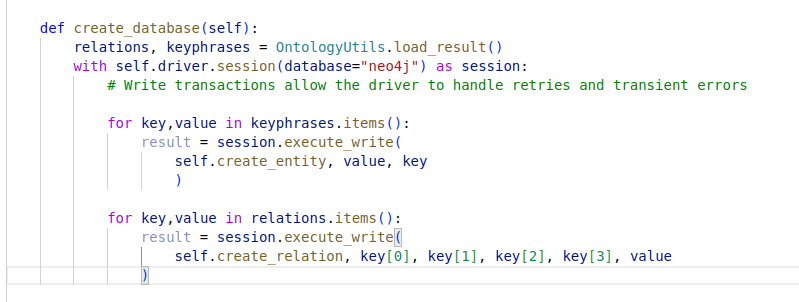
\includegraphics[scale=0.5]{../images/createdatabase}
    \end{center}
	
	La generación de los nodos como entidades la realizamos con las siguientes consulta:
	
	 \begin{center}
		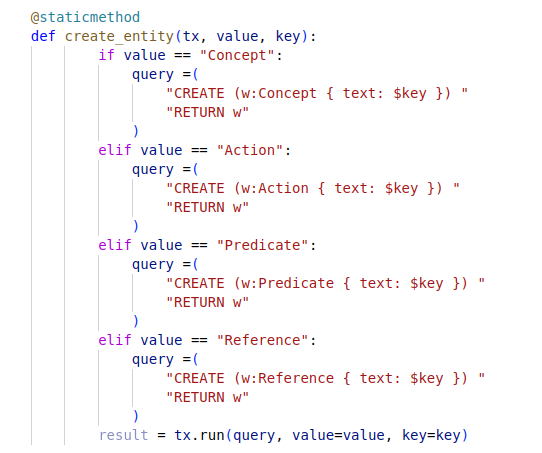
\includegraphics[scale=0.5]{../images/imageEntities}
	\end{center}
	
	Para la creación de las relaciones entre los nodos utilizamos la consulta:
	
	 \begin{center}
		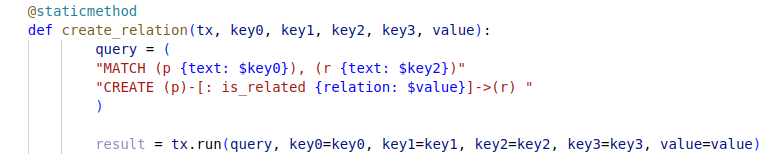
\includegraphics[scale=0.5]{../images/imageRelations}
	\end{center}

	El método a continuaci\'on realiza una consulta para conocer las causas de alguna enfermedad de interés:
	
	\begin{center}
		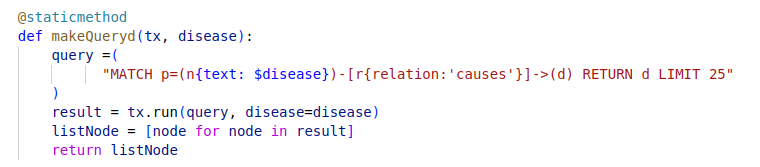
\includegraphics[scale=0.5]{../images/imageQuery}
	\end{center}

	En esta imagen podemos ver los resultado obtenidos al realizar la consulta para conocer las causas del covid-19:
	
	\begin{center}
		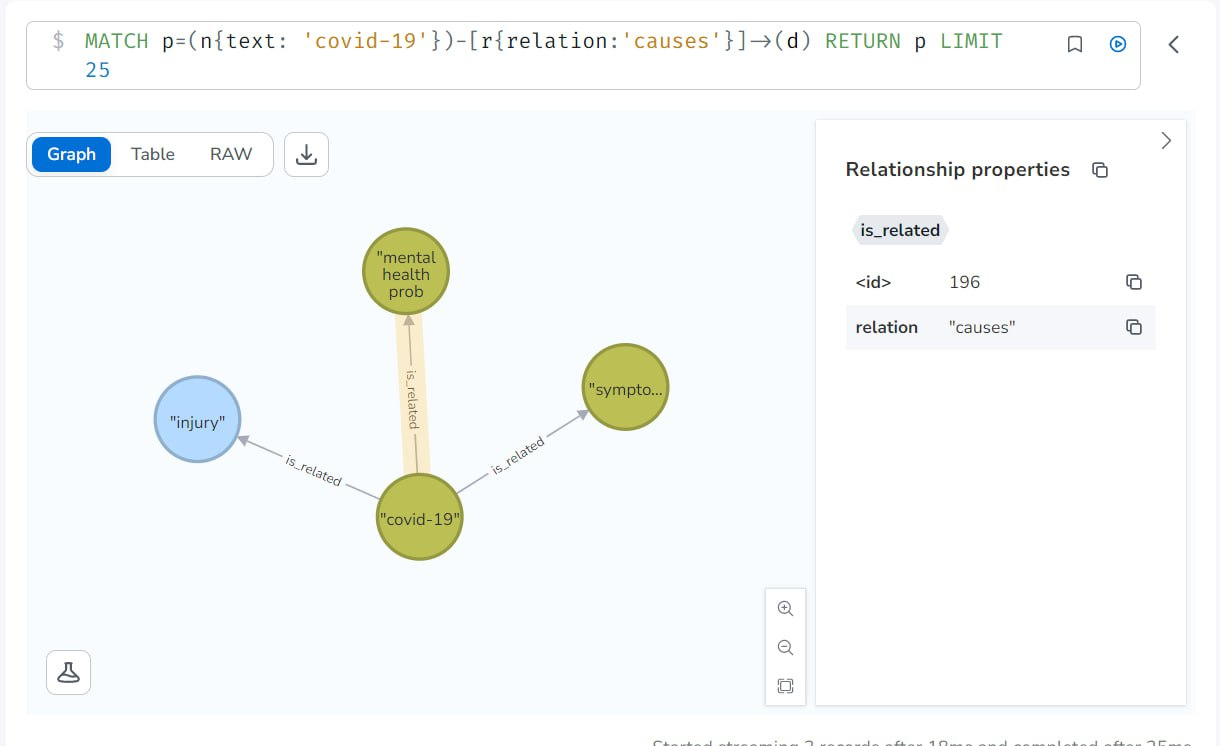
\includegraphics[scale=0.5]{../images/imagecons}
		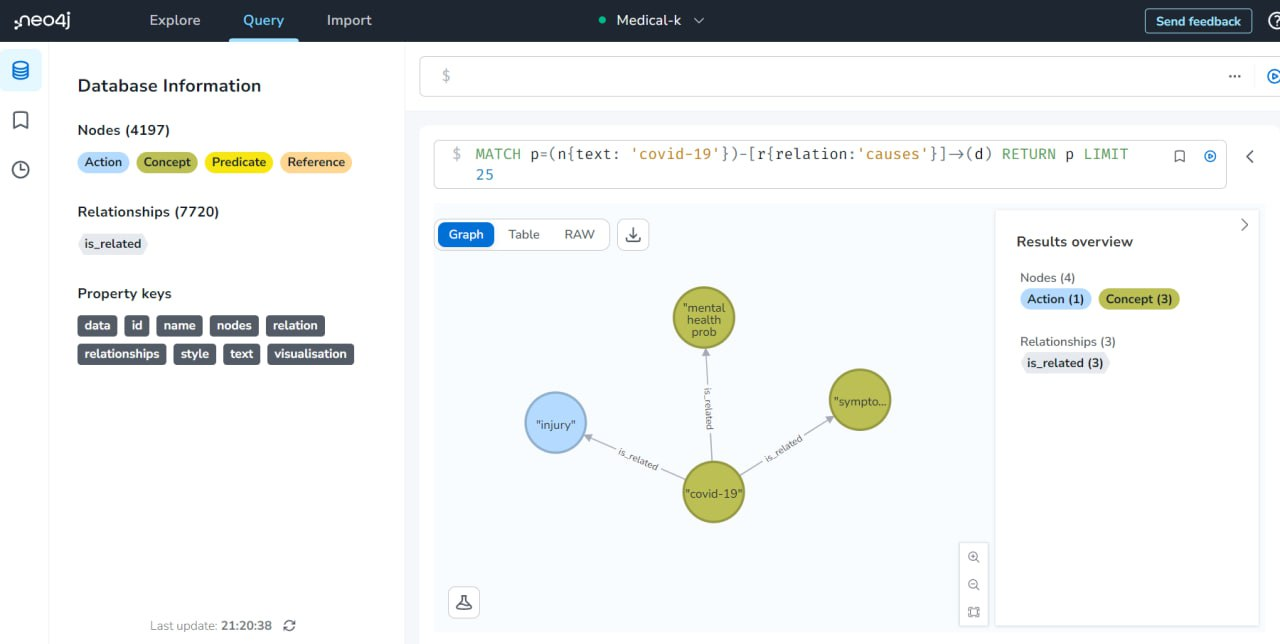
\includegraphics[scale=0.5]{../images/imagecons1}
		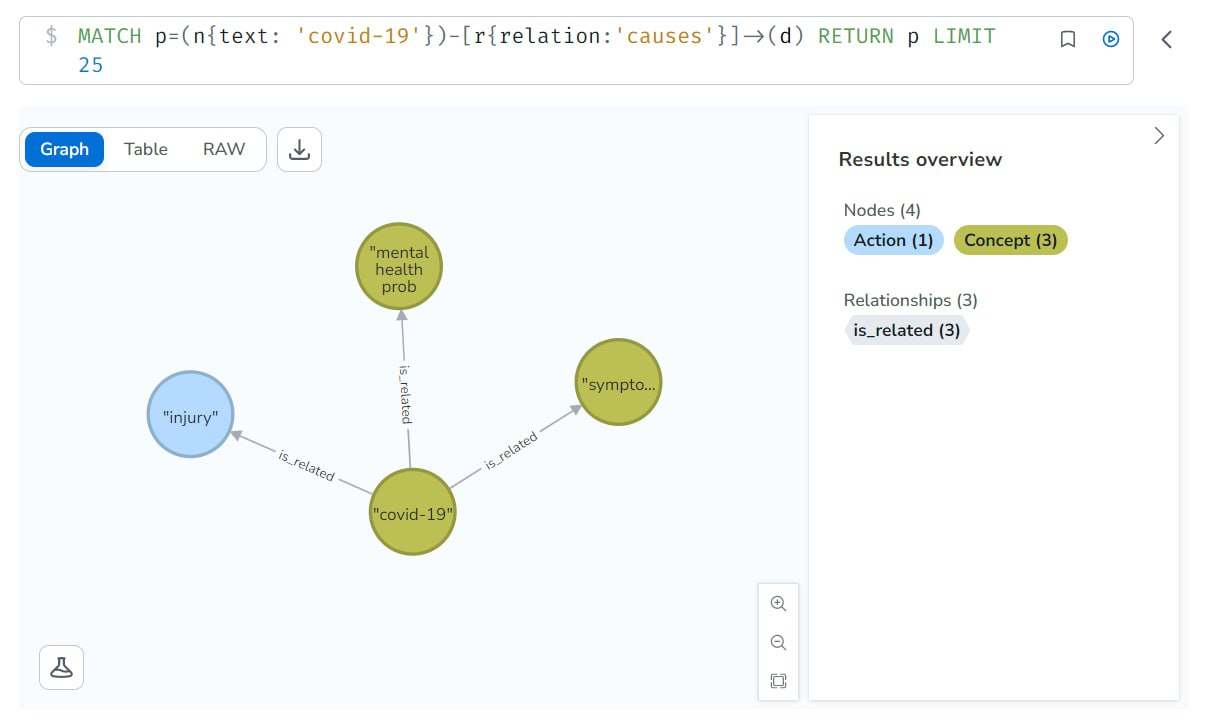
\includegraphics[scale=0.5]{../images/imageconsulta}
	\end{center}

	\section{Resultados}
	
	La siguiente tabla muestra una comparaci\'on del rendimiento de los diferentes modelos implementados, en las distintas tareas abordadas, utilizando como m\'etricas las explicadas en [\ref{evaluacion}].
	\selectlanguage{spanish}
	\begin{table}[htb]
		\centering
		\begin{tabular}{|c|c|c|c|c|}
			\hline
			\textbf{Modelo} & \textbf{Problema} & \textbf{Precisi\'on} & \textbf{Recobrado} & \textbf{F1} \\
			\hline
			\multirow{3}{*}{\textbf{BiLSTM}} & NER & 0.5583 & 0.5613 & 0.5598 \\
			\cline{2-5}
			& RE & 0.06451 & 0.03317 & 0.04381 \\
			\cline{2-5}
			& NER + RE & 0.36909 & 0.30406 & 0.3334 \\
			\hline
		\textbf{BERT} & NER & 1.0 & 0.8375 & 0.455782 \\
			\hline
			\multirow{2}{*}{\textbf{T5}} & NER & 0.535304 & 0.551253 & 0.397562 \\
			\cline{2-5}
			& RE & 0.68838 & 0.1129 & 0.09699 \\
			\hline
			\multirow{3}{*}{\textbf{GPT3}} & NER & 0.41744 & 0.32445 & 0.36512 \\
			\cline{2-5}
			& RE & 0.11374 & 0.061068 & 0.07947 \\
			\cline{2-5}
			& NER + RE & 0.2969 & 0.19602 & 0.23617 \\
			\hline
		
			
		\end{tabular}
		\caption{Comparaci\'on de los resultados de los modelos.}
		\label{resultados}
	\end{table}

	Basándonos en las definiciones de precisión, recobrado y medida F1, se pueden interpretar los resultados obtenidos para los diferentes modelos en las tareas de NER, RE y la combinación de ambas de la siguiente manera:
	
	\begin{itemize}
		\item En la tarea \textbf{NER}, el modelo BiLSTM detect\'o correctamente el 55.83\% de las entidades nombradas y fue capaz de recuperar el 56.13\% de todas las entidades nombradas presentes en el conjunto de datos. El valor de la medida F1, refleja un equilibrio entre la precisi\'on y el recobrado en este modelo y en el modelo T5. Por otro lado, BERT demostr\'o una alta precisi\'on, lo que indica que todas las entidades nombradas detectadas por el modelo fueron correctas, sin embargo, el recobrado fue de 0.8375, lo que implica que el modelo no logró recuperar el 100\% de las entidades nombradas presentes en el conjunto de datos. Por \'ultimo, el modelo GPT3 con medida F1 de 0.36512, tuvo un un rendimiento moderado en la detección de entidades nombradas. El mejor modelo en esta tarea fue el BiLSTM como se observa en la Figura \ref{NER}.
		\item En la tarea \textbf{RE}, los modelos BiLSTM, T5 y GPT3 tuvieron como valor de medida F1 0.04381, 0.09699 y 0.07947, respectivamente, lo que muestra un bajo rendimiento en la extracción de relaciones. Aunque los resultados reflejan un desempeño limitado en esta tarea, el modelo con mayor valor de F1 fue el T5 (Ver Figura \ref{RE}).
		\item En la \textbf{combinaci\'on de ambas tarea}, el modelo BiLSTM tuvo medida F1 igual a 0.3334, lo cual indica que el modelo tuvo dificultades para lograr un rendimiento equilibrado en ambas tareas, obteniendo una precisión moderada pero un recobrado bajo. Por otra parte, la medida F1 del modelo GPT3 fue de 0.23617, que indica un rendimiento bajo en la extracción de entidades y relaciones. En esta tarea el modelo con mejor rendimiento fue el BiLSTM (Ver Figura \ref{NR}).
	\end{itemize}
	 
	 	
	\begin{figure}[h]
		\centering
		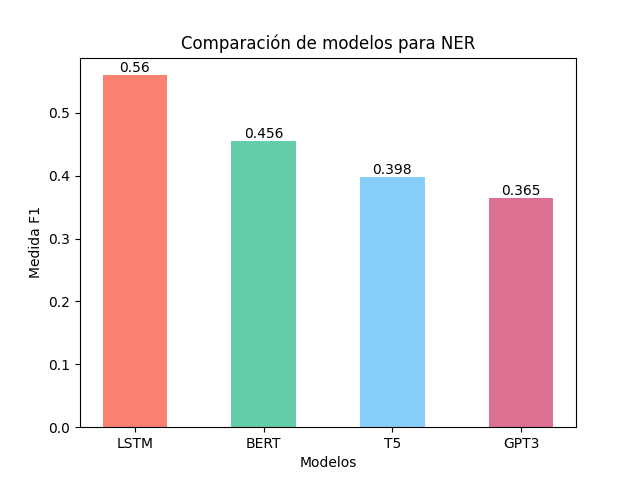
\includegraphics[scale=0.5]{../images/NER_bar}
		\caption{Gr\'afica de barra con los valores de la medida F1 de los modelos evaluados para el problema NER.}
		\label{NER}
	\end{figure}

		\begin{figure}[h!]
		\centering
		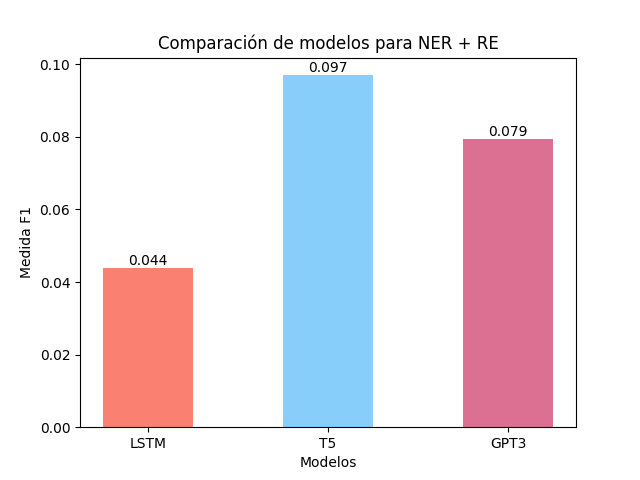
\includegraphics[scale=0.5]{../images/RE_bar}
		\caption{Gr\'afica de barra con los valores de la medida F1 de los modelos evaluados para el problema RE.}
		\label{RE}
	\end{figure}

	
	\begin{figure}[h]
		\centering
		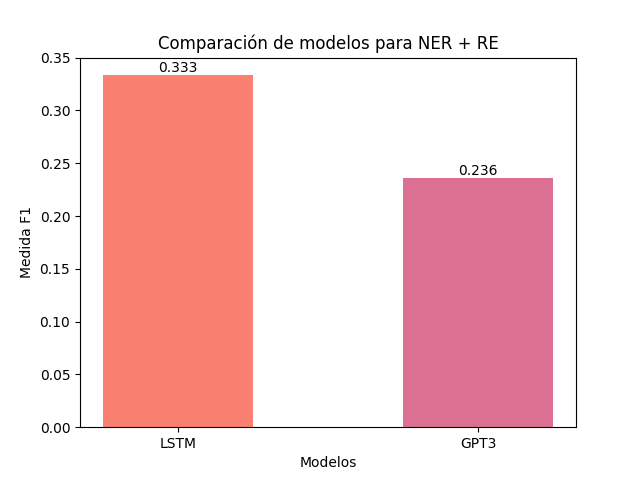
\includegraphics[scale=0.5]{../images/NER_RE_bar}
		\caption{Gr\'afica de barra con los valores de la medida F1 de los modelos evaluados para el problema NER + RE.}
		\label{NR}
	\end{figure}
	
	En general, se puede observar que cada modelo tiene fortalezas y debilidades en las diferentes tareas. Algunos modelos muestran un rendimiento prometedor en la tarea de NER, mientras que otros tienen un mejor desempeño en la tarea de RE. La combinación de ambas tareas también muestra resultados variables.
	
	\section{Conclusiones}
	
	En conclusión, este art\'iculo presenta un estudio sobre el descubrimiento de conocimiento médico utilizando el corpus de HealthKD. Se adoptó un enfoque basado en el reconocimiento de entidades y la extracción de relaciones para identificar y comprender la información relevante en textos médicos.
	
	Se implementaron cuatro modelos diferentes: BiLSTM, BERT, T5 y GPT3, con el objetivo de evaluar su desempeño en las tareas de NER, RE y la combinación de ambas. Tras analizar los resultados obtenidos, se pudo determinar que el modelo BiLSTM fue el que demostró el mejor rendimiento global.
	
	En la resoluci\'on del problema de NER, el modelo BiLSTM alcanzó una precisión, recobrado y F1 superiores en comparación con los otros modelos. Esto significa que logró identificar con mayor precisión y recobrar un mayor número de entidades médicas relevantes en los textos. En cuanto a la tarea de RE, si bien ninguno de los modelos obtuvo un rendimiento excepcional, el modelo BiLSTM mostró un desempeño comparativamente mejor en términos de F1.
	
	Comparado con los otros modelos, BiLSTM demostró una mejor capacidad para capturar y clasificar entidades médicas, lo que es fundamental para el descubrimiento de conocimiento en el campo de la medicina. Sin embargo, se debe tener en cuenta que cada modelo tiene sus fortalezas y debilidades, y el rendimiento puede variar según el conjunto de datos y las características específicas de la tarea. No obstante, estos resultados pueden servir como base para futuras investigaciones y desarrollos en el campo de la extracción de conocimiento médico y contribuir a la mejora de la atención médica y la toma de decisiones clínicas.
	
	
	

	
	\section{Recomendaciones}
	
	
	Basado en los resultados y el análisis realizado en este informe sobre el descubrimiento de conocimiento médico utilizando enfoques de NER y RE, se pueden hacer las siguientes recomendaciones:
	
	\begin{itemize}
		\item Experimentar con modelos más nuevos y potentes: A medida que avanza la investigación en el campo del aprendizaje automático, surgen constantemente nuevos modelos y arquitecturas. Se recomienda explorar modelos más recientes y potentes, como Transformer-based models, que han demostrado un gran rendimiento en diversas tareas de procesamiento de lenguaje natural. Estos modelos pueden ayudar a mejorar la precisión y el recobrado en el descubrimiento de conocimiento médico.
		\item Mejora de los datos de entrenamiento: Los modelos de aprendizaje automático dependen en gran medida de la calidad y cantidad de los datos de entrenamiento. Se recomienda mejorar y ampliar el conjunto de datos utilizado en este estudio. Esto puede implicar la recopilación de más datos etiquetados y la inclusión de diferentes dominios y fuentes de información médica para capturar una mayor variedad de entidades y relaciones.
		\item Pruebas con diferentes combinaciones de modelos: En lugar de utilizar un solo modelo, se sugiere explorar diferentes combinaciones de modelos y técnicas. Por ejemplo, se pueden combinar ensembles de modelos NER y RE para aprovechar las fortalezas de cada uno. También se pueden explorar enfoques de transfer learning para aprovechar los conocimientos aprendidos por un modelo en una tarea y aplicarlos en otra.
		\item Explorar técnicas de preprocesamiento de texto avanzadas: El preprocesamiento de texto es una etapa crucial en el procesamiento de lenguaje natural. Se recomienda explorar técnicas avanzadas de preprocesamiento, como lematización, stemming, eliminación de stopwords y normalización de texto, para mejorar la calidad de los datos de entrada y reducir el ruido en los resultados.
		\item Añadir un preprocesamiento de las entidades y conceptos: Antes de rellenar la base de datos de neo4j, podría sería 
		útil realizar un procesamiento de los datos obtenidos, para que no existan dos entidades que son iguales, por ejemplo se encuentran escritas de manera diferente(errores ortográficos)
	\end{itemize}
	
%-Vicomtech at eHealth-KD Challenge 2021: Deep Learning Approaches to Model Health-related Text in Spanish
%
%- UH-MMM at eHealth-KD Challenge 2021.
%
%- IXA at eHealth-KD Challenge 2021: Generic Sequence Labelling as Relation Extraction Approach
%
%- Documentación oficial de [Spacy](https://spacy.io/api/doc).
%
%- Documentación oficial de [T5](https://huggingface.co/transformers/v4.11.3/model\_doc/t5.html).
%   	
	\begin{thebibliography}
		a
		\bibitem{bert2} Andres, Edgar. \emph{IXA at eHealth-KD Challenge 2021: Generic Sequence Labelling as Relation Extraction Approach}.
		\bibitem{bert} Devlin, Jacob, Chang, Ming-Wei, Lee, Kenton y Toutanova, Kristina. \emph{BERT: Pre-training of Deep Bidirectional Transformers for Language Understanding}.
		\bibitem{bert1} Garcıa-Pablos, Aitor, Perez, Naiara y Cuadros, Montse. \emph{Vicomtech at eHealth-KD Challenge 2021: Deep Learning Approaches to Model Health-related Text in Spanish}. 
		\bibitem{gpt3} Hu, Yan, Ameer, Iqra, Zuo, Xu y otros. \emph{Zero-shot Clinical Entity Recognition using ChatGPT}.
		\bibitem{bilstm1} Monteagudo-Garcıa, Loraine, Marrero-Santos, Amanda, Santiago, Manuel y Canizares-Dıaz, Hian. \emph{UH-MMM at eHealth-KD Challenge 2021}. 
		\bibitem{corpus} Piad-Morffis, Alejandro, Gutiérrez, Yoan y Muñoz, Rafael. \emph{A corpus to support eHealth Knowledge Discovery technologies}. Journal of Biomedical Informatics. 2019.		 
		\bibitem{attention} Vaswani, Ashish, Shazeer, Noam, Parmar, Niki, Uszkoreit, Jakob y Jones, Llion. \emph{Attention Is All You Need}.2017.
		
		
		
	
		
		
	\end{thebibliography}



\end{document}


